\documentclass[11pt]{article}
\usepackage[utf8]{inputenc}
\usepackage{amsmath, amssymb}
\usepackage{geometry}
\usepackage{listings}
\usepackage{xcolor}
\usepackage{tabularx}
\usepackage{booktabs}
\usepackage{hyperref}
\usepackage{tikz}
\usetikzlibrary{shapes, arrows.meta, positioning, calc, decorations.pathreplacing}

\geometry{a4paper, margin=1in}

\definecolor{codegray}{rgb}{0.5,0.5,0.5}
\definecolor{codepurple}{rgb}{0.58,0,0.82}
\definecolor{backcolour}{rgb}{0.95,0.95,0.92}
\definecolor{blockbg}{RGB}{31,38,64}

\lstset{
    language=Python,
    backgroundcolor=\color{backcolour},
    commentstyle=\color{codegray},
    keywordstyle=\color{magenta},
    stringstyle=\color{codepurple},
    basicstyle=\ttfamily\small,
    breaklines=true,
    showstringspaces=false
}

\title{Quantum Dynamics Lab: Mini Fourier Neural Operator \\ \large Problem Set \& Implementation Guide}
\author{VB}
\date{\today}

\begin{document}

\maketitle

\section*{Problem 0: Start the engine}

Consider the files given.
\begin{center}
\renewcommand{\arraystretch}{1.5}
\begin{tabularx}{\textwidth}{@{} >{\bfseries\raggedright\arraybackslash}p{5.5cm} X @{}}
\toprule
\textcolor{blue}{Filename} & \textcolor{blue}{Purpose} \\ \midrule
\multicolumn{2}{@{}l}{\textbf{Direct Interaction}} \\ \midrule
\lstinline|implementation_tasks.py| & \textcolor{red}{Here you write your code.} Contains the architecture of the neural operator intended for student implementation. You can add your own \lstinline|unittest.TestCase| classes at the bottom and run \lstinline|python implementation_tasks.py| to execute them. \\
\lstinline|lab_dashboard.py| & \textcolor{red}{This file you run.} A dedicated educational sandbox for training and testing your FNO model against the numerical simulator ground truth. \\
\bottomrule
\end{tabularx}
\end{center}

\textbf{Prerequisites:} You will need to install the basic dependencies via \lstinline|pip install -r requirements.txt|. Then, run \lstinline|python install_pytorch.py| which will automatically detect your hardware (Mac, new GPU, old GPU, or CPU) and install the correct PyTorch version for your device.

\section*{PyTorch Mini-Reference}

\begin{center}
\renewcommand{\arraystretch}{1.3}
\begin{tabularx}{\textwidth}{@{} >{\ttfamily\small}l X @{}}
\toprule
\textcolor{blue}{PyTorch} & \textcolor{blue}{NumPy equivalent / Notes} \\ \midrule
import torch & import numpy as np \\
torch.tensor(arr) & Creates a tensor from a NumPy array \\
torch.fft.rfft(t) / irfft(t) & Real-valued FFT and inverse \\
torch.einsum("bix,iox->box", A, B) & Einstein summation (batched matmul) \\
nn.Parameter(tensor) & Learnable parameter (tracked by optimizer) \\
nn.Linear(in, out) & Fully connected layer \\
nn.Conv1d(in, out, kernel=1) & Pointwise 1D convolution \\
F.gelu(x) & GeLU activation function \\
\bottomrule
\end{tabularx}
\end{center}

\section*{Task 1: Spectral Convolution}

\subsubsection*{Mathematical part}
The split-step Fourier method is exact, but sequential: predicting $\psi(x, t)$ requires stepping through every intermediate time step $\Delta t$. A \textbf{Fourier Neural Operator} (FNO) learns to approximate the time-evolution operator directly, effectively allowing $\mathcal{O}(1)$ inference to leap forward to any target time.

Traditional neural networks use discrete convolutions, which are limited by small local receptive fields. The Schrödinger equation is non-local; a wave packet spreading globally cannot be captured easily by local kernels. A general integral operator $(\mathcal{K}v)(x) = \int \kappa(x, y)\,v(y)\,dy$ has a global receptive field, but requires learning $\mathcal{O}(N^2)$ parameters.

However, if the kernel is translation-invariant ($\kappa(x, y) = \kappa(x-y)$), the \textbf{Convolution Theorem} gives:
$$
\mathcal{F}[\mathcal{K}(v)](k) = \hat{\kappa}(k) \cdot \hat{v}(k)
$$
A global integral convolution becomes a simple pointwise multiplication in Fourier space! The FNO explicitly leverages this by learning the Fourier-space kernel $R(k)$ directly. We discard the higher-frequency modes, keeping only $k_{\text{max}}$ modes, effectively creating a low-pass filter that acts as a continuous, mesh-free operator.

\begin{center}
\resizebox{0.9\linewidth}{!}{
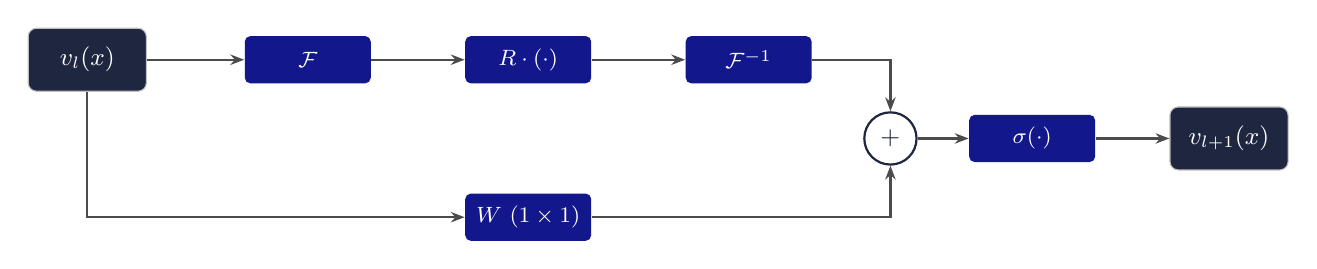
\begin{tikzpicture}[
  box/.style={rectangle, rounded corners=3pt, minimum width=1.5cm, minimum height=0.8cm, draw=gray!50, fill=blockbg, text=white, font=\small, align=center},
  op/.style={rectangle, rounded corners=2pt, minimum width=1.6cm, minimum height=0.6cm, fill=blockbg!60!blue, text=white, font=\footnotesize},
  arr/.style={-{Stealth[length=5pt]}, thick, black!70}
]
% Top path (spectral)
\node[box] (vin) at (0,1) {$v_l(x)$};
\node[op] (fft) at (2.8,1) {$\mathcal{F}$};
\node[op] (R) at (5.6,1) {$R \cdot (\cdot)$};
\node[op] (ifft) at (8.4,1) {$\mathcal{F}^{-1}$};
\node[op] (sigma) at (12,0) {$\sigma(\cdot)$};
\node[box] (vout) at (14.5,0) {$v_{l+1}(x)$};

% Bottom path (local)
\node[op] (W) at (5.6,-1) {$W$ ($1\times 1$)};

% Plus
\node[circle, draw=blockbg, fill=white, thick, minimum size=0.5cm, font=\small, text=blockbg] (plus) at (10.2,0) {$+$};

\draw[arr] (vin) -- (fft);
\draw[arr] (fft) -- (R);
\draw[arr] (R) -- (ifft);
\draw[arr] (ifft) -| (plus);
\draw[arr] (vin) |- (W);
\draw[arr] (W) -| (plus);
\draw[arr] (plus) -- (sigma);
\draw[arr] (sigma) -- (vout);
\end{tikzpicture}
}
\end{center}

\subsubsection*{Implementation part}
\textbf{Implement:}
1. The \lstinline|__init__| method is provided for you. Take a moment to see how it scales and initializes the complex weights \lstinline|self.weights|.
2. \lstinline|SpectralConv1d.forward(self, x)|: 
    - Compute the real FFT along the spatial dimension.
    - Create a zero-tensor of the correct size in Fourier space.
    - Use \lstinline|torch.einsum| to multiply the first \lstinline|modes| of the input with your learned weights, and store the result in the zero-tensor.
    - Compute the inverse real FFT and return it.

\section*{Task 2: The PINNs Trick}

\subsubsection*{Mathematical part}
The FNO needs to predict the state at an arbitrary continuous time $t$. However, deep neural networks struggle to learn high-frequency periodic mappings directly from a single scalar value. 

To solve this, we use a trick common in Physics-Informed Neural Networks (PINNs) and NeRFs: we embed $t$ into a high-dimensional space using sinusoidal \textbf{Fourier Features}. Instead of giving the network the raw number $t=5.3$, we give it $\sin(f \cdot t)$ and $\cos(f \cdot t)$ for a spectrum of frequencies $f \in \{1, 2, 4, 8, 16\}$. This provides the network with multiple "clocks" ticking at different speeds, making it trivial for linear layers to construct the necessary phase oscillations.

\subsubsection*{Implementation part}
\textbf{Implement:}
1. \lstinline|generate_temporal_features(t, N_x)|:
    - Iterate over the frequencies $f \in \{1, 2, 4, 8, 16\}$.
    - For each frequency, compute $\sin(f \cdot t)$ and $\cos(f \cdot t)$, and append them to a list.
    - Concatenate the list along the last dimension to create a tensor of shape \lstinline|(batch, 10)|.
    - Since the next layer is a pointwise convolution across the spatial grid, expand this time embedding to every point in space: \lstinline|t_feats.unsqueeze(1).expand(batch, N_x, 10)|.

\section*{Task 3: Full FNO Architecture}

\subsubsection*{Mathematical part}
Now we assemble the entire architecture. To keep the deep learning pure, the physics visualization sandbox will automatically prepare a \textbf{14-channel grid} for you:
\begin{itemize}
    \item $V(x)$ normalized to $[-0.1, 0.1]$ (1 channel)
    \item The spatial coordinates $x$ (1 channel)
    \item The temporal Fourier features you generated in Problem 2 (10 channels)
    \item $\text{Re}[\psi_0(x)]$ and $\text{Im}[\psi_0(x)]$ (2 channels)
\end{itemize}

The network simply lifts these 14 features into a wide channel space, applies five Fourier spectral blocks, and projects back down to 3 output channels: $\text{Re}[\psi]$, $\text{Im}[\psi]$, and $|\psi|^2$.

\begin{center}
\resizebox{0.95\linewidth}{!}{
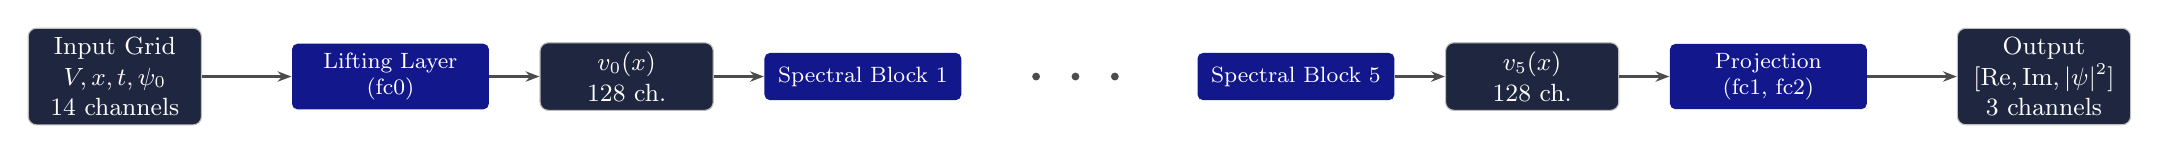
\begin{tikzpicture}[
  box/.style={rectangle, rounded corners=3pt, minimum width=2.2cm, minimum height=0.8cm, draw=gray!50, fill=blockbg, text=white, font=\small, align=center},
  op/.style={rectangle, rounded corners=2pt, minimum width=2.5cm, minimum height=0.6cm, fill=blockbg!60!blue, text=white, font=\footnotesize, align=center},
  arr/.style={-{Stealth[length=5pt]}, thick, black!70}
]
\node[box] (in) at (0,0) {Input Grid\\$V, x, t, \psi_0$\\14 channels};
\node[op] (lift) at (3.5,0) {Lifting Layer\\(fc0)};
\node[box] (h0) at (6.5,0) {$v_0(x)$\\128 ch.};

\node[op] (block1) at (9.5,0) {Spectral Block 1};
\node[circle, fill=black!70, inner sep=1pt] (d1) at (11.7, 0) {};
\node[circle, fill=black!70, inner sep=1pt] (d2) at (12.2, 0) {};
\node[circle, fill=black!70, inner sep=1pt] (d3) at (12.7, 0) {};
\node[op] (block5) at (15,0) {Spectral Block 5};

\node[box] (h5) at (18,0) {$v_5(x)$\\128 ch.};
\node[op] (proj) at (21,0) {Projection\\(fc1, fc2)};
\node[box] (out) at (24.5,0) {Output\\{}$[\text{Re}, \text{Im}, |\psi|^2]$\\3 channels};

\draw[arr] (in) -- (lift);
\draw[arr] (lift) -- (h0);
\draw[arr] (h0) -- (block1);
\draw[arr] (block5) -- (h5);
\draw[arr] (h5) -- (proj);
\draw[arr] (proj) -- (out);
\end{tikzpicture}
}
\end{center}

\subsubsection*{Implementation part}
\textbf{Implement:}
1. The \lstinline|__init__| method is already provided for you so you don't have to write out PyTorch boilerplate. Take a moment to read how the 14-channel input is mapped to the hidden width, and how the spectral blocks are assembled.
2. \lstinline|FNO1d.forward(self, V_in, x_coord, t, psi0_re, psi0_im)|:
    - \textbf{Consciously} call your \lstinline|generate_temporal_features(t, N_x)| to get the 10-channel \lstinline|t_in|.
    - \textbf{Consciously} stack \lstinline|V_in|, \lstinline|x_coord|, \lstinline|t_in|, \lstinline|psi0_re|, and \lstinline|psi0_im| along the last dimension using \lstinline|torch.cat| to build the 14-channel \lstinline|grid|.
    - Pass the 14-channel \lstinline|grid| through the lifting layer.
    - PyTorch convolutions expect inputs of shape \lstinline|(batch, channels, spatial)|. Permute your dimensions accordingly.
    - Apply the five spectral blocks (SpectralConv + Conv1d + GeLU).
    - Permute back to \lstinline|(batch, spatial, channels)|.
    - Apply the projection layers (Linear + GeLU + Linear) to return the final 3-channel output.

Once implemented, run \lstinline|python lab_dashboard.py| to watch the model learn to predict wave packet propagation!

\section*{\textcolor{red}{Submission}}

Submit the file \texttt{implementation\_tasks.py}.

\end{document}
